% === Notes from Elvis ===

%%%%%%%%%%%%%%%%%%%%%%%%%%%%%%%%%%%%%%%%%%%%%%%%%%%%%%%%%%%%%%%%%%%%%%%%%%%%%%%%
% The above line is 80 characters long. Try to keep it under this width.

% There are 3 ways of highlighting:
%  o \texttt
%      o Folders
%      o Files
%      o Program names
%  o \emph
%      o Company names
%      o New concepts that are introduced
%  o \textcode (\texttt with grey background)
%      o Commands
%      o Command output

%\chapter
%    \section
%        \subsection
%            \subsubsection
%            \paragraph

% === Setup ===

% Needed and Layout
\documentclass[a4paper,11pt]{report}
\usepackage[utf8]{inputenc} % utf8 encoding
\usepackage{amsfonts}
\usepackage[T1]{fontenc} % use for allowing < and > in cleartext
\usepackage[margin=2.5cm]{geometry}

% Lists
\usepackage{verbatim}   % useful for program listings
\usepackage{enumitem}
\usepackage[ampersand]{easylist}

% Creating more compact lists
\let\olditemize\itemize
\renewcommand{\itemize}{
    \olditemize
    \setlength{\itemsep}{1pt}
    \setlength{\parskip}{0pt}
    \setlength{\parsep}{0pt}
}


% Creating shortcut for \footnote{\fn}
\newcommand{\f}{\footnote{\fn}}


% Creating shortcut for Red Text
\newcommand{\rt}[1]{
    {\color{red}#1}}

% Creating shortcut for Grey Text
\newcommand{\gt}[1]{
    {\color{gray}#1}}

% Trying to create a column tyupe that aligns the dots
\usepackage{dcolumn}
\newcolumntype{d}{D{.}{.}{-1} }


% Creating my own inline code font
\newcommand{\textcode}[1]{\fboxsep=1pt\texttt{\colorbox{gray!20}{#1}}}
\newcommand{\textred}[1]{\fboxsep=1pt{\colorbox{red!20}{#1}}}
\newcommand{\textgreen}[1]{\fboxsep=1pt{\colorbox{green!20}{#1}}}
\newcommand{\textgray}[1]{\fboxsep=1pt{\colorbox{gray!20}{#1}}}
\newcommand{\textblue}[1]{\fboxsep=1pt{\colorbox{blue!20}{#1}}}
    \def \redmid{gray!20}
    \def \reddark{gray!40}
\newcommand{\textreddark}[1]{\fboxsep=1pt{\colorbox{\reddark}{#1}}}
\newcommand{\textredmid}[1]{\fboxsep=1pt{\colorbox{\redmid}{#1}}}

% Recreating the figure thingy
\newcommand{\figa}{
    \begin{figure}[!htpb]
    \centering
}
\newcommand{\figb}[2]{
    \caption{#1}
    \label{#2}
    \end{figure}
}
\newcommand{\figc}{
    \end{figure}
}

\usepackage{subfigure}


% Math
\usepackage{mathtools}   % need for subequations
\usepackage{xfrac}       % Fractions  like 1/4 via \sfrac

% Graphics
\usepackage{graphicx}   % need for figures
\usepackage{color}      % use if color is used in text 
\usepackage[table]{xcolor}     % use for table and text background color
\usepackage{tikz}
\usetikzlibrary{arrows}
\usepackage{float}

% Other
\usepackage{todonotes}
\usepackage{pdfpages}
\usepackage{latexsym}
\usepackage{fixltx2e}    % use for textsubscript
\usepackage{datetime}    % for the \currenttime
\usepackage[titletoc,title]{appendix}
\usepackage[framemethod=tikz]{mdframed}
\usepackage[titletoc,title]{appendix}
\usepackage{epstopdf}

% Code listing
\usepackage{listings} % For inserting code from file (I think)

% Citations and refs
\usepackage{hyperref} % Citations and refs are links
\hypersetup{colorlinks=true,citecolor=blue}
\usepackage{cite}


% URLs 
\usepackage{url}
\usepackage[hypcap=true]{caption}


% for the \lstinputlisting for code blocks
\definecolor{codegreen}{rgb}{0,0.6,0}
\definecolor{codegray}{rgb}{0.5,0.5,0.5}
\definecolor{codepurple}{rgb}{0.58,0,0.82}
\definecolor{backcolour}{rgb}{1.0,1.0,1.0}

\lstdefinestyle{mystyle}{
  backgroundcolor=\color{backcolour},   
  commentstyle=\color{codegreen},
  keywordstyle=\color{magenta},
  numberstyle=\tiny\color{codegray},
  stringstyle=\color{codepurple},
  basicstyle=\ttfamily\footnotesize,
  breakatwhitespace=false,         
  breaklines=true,                 
  captionpos=b,                    
  keepspaces=true,                 
  numbers=left,                    
  numbersep=5pt,                  
  showspaces=false,                
  showstringspaces=false,
  showtabs=false,                  
  tabsize=2,
  emph={ifdef,endif,\#},
  emphstyle={\color{red}}
}


\lstset{style=mystyle}

\begin{document}

% Configuration
\setlength{\parindent}{0cm}
\setlength{\unitlength}{1mm}

% Front Page
\date{September 1st 2015\\ IT University of Copenhagen}
\title{A Quantitative Analysis of Variability Warnings in Linux \\ Draft: 
    \today~\currenttime}
\author{Elvis Flesborg\\
\texttt{efle@itu.dk}}
\clearpage\maketitle
\thispagestyle{empty}
\newpage

%%%%%%%%%%%%%%%%%%%%%%%%%%%%%%%%%%%%%%%%%%%%%%%%%%%%%%%%%%%%%%%%%%%%%%%%%%%%%%%%
%                           TABLE OF CONTENTS
%%%%%%%%%%%%%%%%%%%%%%%%%%%%%%%%%%%%%%%%%%%%%%%%%%%%%%%%%%%%%%%%%%%%%%%%%%%%%%%%
\tableofcontents
\thispagestyle{empty}



\newpage

\setcounter{page}{1}


            %%%%%%%%%%%%%%%%%%%%%%%%%%%%%%%%%%%%%%%%%%%%%%%%%%%
            %        ABSTRACT
            %%%%%%%%%%%%%%%%%%%%%%%%%%%%%%%%%%%%%%%%%%%%%%%%%%%
            \begin{abstract}

The Linux kernel is the largest open source project to implement variability. It
has more than 14,000 options in total that can be switched on and off. This can 
generate more variants of the Linux kernel, than there are atoms in the 
universe, and bugs can be harder to find with the extra dimension of 
variability.
\\

In this project, a sample of these variants are produced and checked for compile
warnings to get an insight in the distribution of warning types, and the 
location of the warnings. The experiment is run both on a stable version of the 
Linux kernel, and an in-development version, which are compared regarding types 
and location of the warnings.



            \end{abstract}


%%%%%%%%%%%%%%%%%%%%%%%%%%%%%%%%%%%%%%%%%%%%%%%%%%%%%%%%%%%%%%%%%%%%%%%%%%%%%%%%
%                           INTRODUCTION
%%%%%%%%%%%%%%%%%%%%%%%%%%%%%%%%%%%%%%%%%%%%%%%%%%%%%%%%%%%%%%%%%%%%%%%%%%%%%%%%
\chapter{Introduction}
Software projects with a high variability rate can be configured, to suit many
needs with the same code base. Possibly the largest open source project, which 
also happens to be the project with the highest variability rate
is the Linux kernel. It contains approximately 10,000 different configuration 
options in the feature model.
\\

The basis for this paper is another  paper: \emph{42 Variability 
Bugs in the Linux Kernel: A Qualitative Analysis}\cite{42bugs}, where bugs in 
the Linux kernel are qualitatively analyzed. In this report, warnings will be 
analysed quantitatively, and will function as a proxy for bugs.
\\

The following contributions will be made: Analysis of distributions of warnings 
in the Linux kernel, comparison of warnings in a stable version of the Linux 
kernel vs.\ an in-development version. Also an analysis of where the warnings 
are located.

% TODO
\iffalse
 v  Large amount of variability
 .  Software Product Lines
 v  Linux Kernel
 v  42 bugs paper
 v  During development (stable vs unstable)
 v  Following contributions:
     v  distribution of warnings in Linux
     v  difference in stable and unstable
     v  distribution of subsystems
 v  Research Questions
\fi




%%%%%%%%%%%%%%%%%%%%%%%%%%%%%%%%%%%%%%%%%%%%%%%%%%%%%%%%%%%%%%%%%%%%%%%%%%%%%%%%
%                           BACKGROUND
%%%%%%%%%%%%%%%%%%%%%%%%%%%%%%%%%%%%%%%%%%%%%%%%%%%%%%%%%%%%%%%%%%%%%%%%%%%%%%%%
\newpage
        \chapter{Background}

            %% VARIABILITY
            \section{Variability}

Many software products are configurable in some way. Configurability creates the 
possibility of tailoring the software to suit different needs. For example 
different kinds of hardware, or different functionalities. 
\\

This is called \emph{variability} in software, and a software product of 
this type is called a \emph{Software Product Line} (SPL). Software products 
with different functionalities (\emph{variants}) can be derived from the same 
source code base, and the code in its entirety is not a valid product\cite[p. 
1]{IntDatSPL}, it has to be configured.
\\

        \def \fn {14,387 across all architectures, with an average of 9,984 per 
        architecture, and 10,335 for the \texttt{x86} architecture, which is used
        in this project.}

Software with a high-degree of variability is usually refered to as 
\emph{Variability-Intensive Systems} or \emph{VISs}. Linux is a \emph{VIS} with 
more than 14,000\f different configuration options, called \emph{features}.
Other examples of \emph{VISs} are \textsc{BusyBox}, \textsc{Eclipse}, 
\textsc{Amazon Elastic Compute Service}, and \textsc{Drupal Content Management 
Framework}\cite[p. 1]{VarTesDrupal} to name a few.
\\

All features in a software product line, and their options and relations are 
described in a \emph{feature model}.

            %%% FEATURE MODELS
            \subsection{Feature Models}

A feature model is a way of representing all the possible configurations - 
\emph{the configuration space}. It contains all the features with their 
respective options and all the constraints and dependencies between the features.

A visualization of a feature model is called a feature diagram, there is an 
example in Figure \ref{featurediagramphone}. The example will be tiny compared 
to that of the Linux kernel. With many thousands of features, the feature model 
of the Linux kernel is too big to fit on a normal sized paper.

Figure \ref{featurediagramphone} depicts a feature model of a phone 
configuration with 10 features, where some are mandatory: \textbf{Screen} and 
\textbf{Calls}, and some are optional: \textbf{GPS} and \textbf{Media}, which has 2
optional features \textbf{Camera} and \textbf{MP3} depending on it.

There is also some choice options \textbf{Color}, \textbf{BW}, and \textbf{High 
Definition} for the screen type, where only one of them may be enabled. 
\textbf{High Definition} is the default choice. A 
cross-tree constraint is also present, which states that \textbf{Media} with 
all of its children can only be enabled if a \textbf{High Definition} screen is 
enabled.

The feature diagram is inspired by \cite{AAFM}, but there is no consensus on a 
unified notation for attributes in feature models\cite{AAFM}. And for there is 
for example no notation in the diagram, that \textbf{High Definition} is the 
default value for the choice clause.

The phone example is inspired by some examples from \cite{SPLOT}, which is an 
online toolbox for variability software that also has a repository of feature 
models and diagrams.



% The feature diagram
% 80 lines down to \figb
\figa
    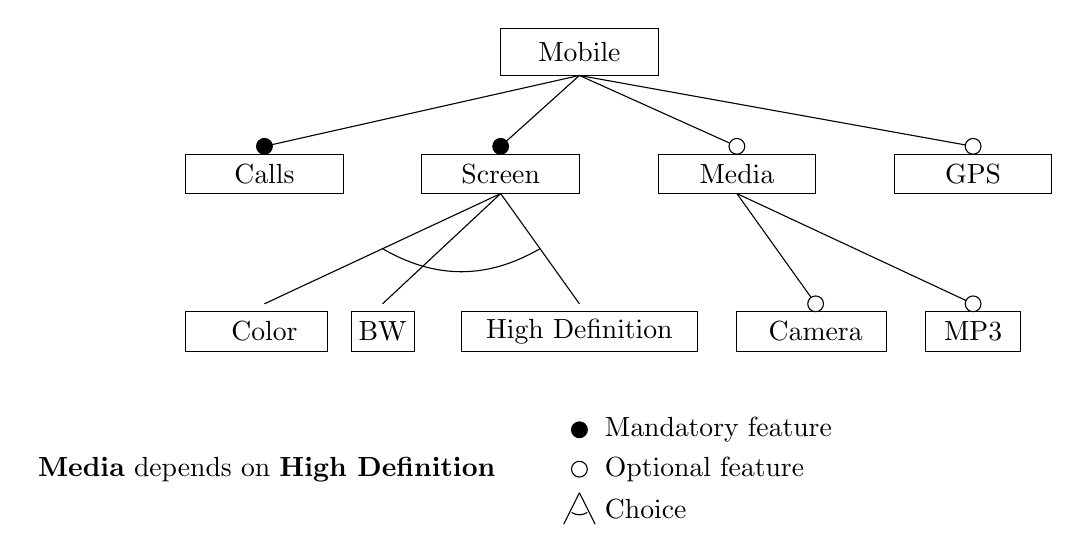
\begin{tikzpicture}
        % The top box
        \draw (3,3) rectangle (5,3.6);
        \draw (4,3.3) node {Mobile};

        % Middle words
        \draw (0.00,1.75) node {Calls};
        \draw (3,1.75) node {Screen};
        \draw (6,1.75) node {Media};
        \draw (9,1.75) node {GPS};

        % Middle edges
        \draw (0,2.1) edge (4,3);
        \draw (3,2.1) edge (4,3);
        \draw (6,2.1) edge (4,3);
        \draw (9,2.1) edge (4,3);

        % Middle dots
        \draw[fill=black] (0,2.1) circle (0.1);
        \draw[fill=black] (3,2.1) circle (0.1);
        \draw[fill=white] (6,2.1) circle (0.1);
        \draw[fill=white] (9,2.1) circle (0.1);

        % Middle boxes
        \draw (-1,1.5) rectangle (1,2);
        \draw (2,1.5) rectangle (4,2);
        \draw (5,1.5) rectangle (7,2);
        \draw (8,1.5) rectangle (10,2);

        % Bottom words
        \draw (0,-0.25) node {Color};
        \draw (1.5,-0.25) node {BW};
        \draw (4,-0.25) node {High Definition};
        \draw (7,-0.25) node {Camera};
        \draw (9,-0.25) node {MP3};

        % Bottom edges
        \draw (0,0.1) edge (3,1.5);
        \draw (1.5,0.1) edge (3,1.5);
        \draw (4,0.1) edge (3,1.5);
        \draw (7,0.1) edge (6,1.5);
        \draw (9,0.1) edge (6,1.5);

        % Bottom dots
        %\draw[fill=white] (0,0.1) circle (0.1);
        %\draw[fill=white] (2,0.1) circle (0.1);
        %\draw[fill=white] (4,0.1) circle (0.1);
        \draw[fill=white] (7,0.1) circle (0.1);
        \draw[fill=white] (9,0.1) circle (0.1);

        % The 'or'
        \draw (1.5,0.8) edge [bend right] (3.5,0.8);

        % Bottom boxes
        \draw (-1,-0.5) rectangle (0.8,0);
        \draw (1.1,-0.5) rectangle (1.9,0);
        \draw (2.5,-0.5) rectangle (5.5,0);
        \draw (6,-0.5) rectangle (7.9,0);
        \draw (8.4,-0.5) rectangle (9.6,0);


        % The legend
        \draw[fill=black] (4,-1.5) circle (0.1);
        \draw[fill=white] (4,-2) circle (0.1);
        \draw[right] (4.2,-1.5) node {Mandatory feature};
        \draw[right] (4.2,-2) node {Optional feature};

        \draw (4.0,-2.3) edge (4.2,-2.7);
        \draw (4.0,-2.3) edge (3.8,-2.7);
        \draw (4.1,-2.55) edge [bend left] (3.9,-2.55);
        \draw[right] (4.2,-2.5) node {Choice};

        % The cross-tree dependency
        \draw[right] (-3, -2) node {\textbf{Media} depends on 
            \textbf{High Definition}};

    \end{tikzpicture}
\figb{A feature diagram of a phone}{featurediagramphone}
% 80 lines up to \figa


The feature diagrams of \emph{VIS}s are typically wide and shallow. The Linux 
kernel feature model hierarchy, for example, is only 8 layers deep\cite[p. 
17]{VarModSSD}.


            %%% BUGS IN VARIABILITY
            \subsection{Bugs In Variability}

Bugs in variability programs do not necessarily generate a bug in every 
variant of the program. A simple example is shown in Figure \ref{lst:varbug}. 
There are only two feature in the feature model: \texttt{A}, and \texttt{B}, 
and thus there are four different configurations for this program; 
\texttt{\{\}}, \texttt{\{A\}}, \texttt{\{B\}}, and \texttt{\{A,B\}}.

The feature model, denoted $\psi_{FM}$, for this example contains four 
configurations, $\kappa_0$, $\kappa_1$, $\kappa_2$, and $\kappa_3$, which can 
be denoted as conjunctions on logic form like this: $\kappa_0 = \neg A \wedge 
\neg B$, and $\kappa_1 = \neg A \wedge B$.
\\

In the variant of the program with configuration $\kappa_0$, the compilation of 
the program will return an \texttt{uninitialized} warning, since the compiler 
never visits the two \textcode{\#ifdef}-clauses. In all other variants of the
program, there will be no warning, because \textcode{var} gets initialized.

\figa
    \subfigure{
    \lstinputlisting[language=C,firstline=3,]{code/varbug.c}
    }
\figb{An example of a program with a variability bug.}{lst:varbug}

            
            %% THE LINUX KERNEL
            \section{The Linux Kernel}

            \def \fn {See the \textcode{README} file in the Linux kernel tree}

The Linux kernel is written by many thousand of people all over 
the world, and has been ported to more than 20 architectures\f, which makes it 
very scalable, it is the operating system that supports the most hardware in
the world\cite{22thbirthday,gkh}.

Its use cases range from small embedded devices like mobile phones and GPSs to 
supercomputers. In fact 98\% of the top 500 supercomputers in the world run a 
Linux distribution\cite{top500}. 
\\

It was first developed in 1991 by \emph{Linus Torvalds}, and has since been 
growing. Today the code base is 19 million lines of code.


            \section{Linux Kernel Development}

            \def \fn {See the \textcode{MAINTAINERS} file in  
            the Linux kernel tree}

The Linux kernel development model is unique in the  way, that it is developed 
by many thousands of people all over the world. According to \cite{gkh}, 
approximately 75\% of the contributions come from companies, and 25\% come from 
individuals. 

There is a hierarchy of people, who are head-maintainers of different parts of 
the kernel\f.


            \subsection*{Stable Releases}

The Linux kernel development cycle has approximately 2$\sfrac{3}{4}$ months 
from one stable release to the next stable release\cite
    {crystalball}.
In the meantime, weekly semi-stable versions are released.

When the top maintainers of the mainline tree think that enough bugs have been 
fixed, a new stable version is created, and the whole process is repeated.


            \subsection*{In-development Releases}

            \def \fn {See the original post about it here: 
            \url{https://lkml.org/lkml/2008/2/11/512}}

During development, new code is added to the in-development version of Linux.
This version is called \emph{linux-next}, and has been the main in-development version
since 2008\f.
\\

            \def \fn {\textsc{git} is a version control system that is created
            by and for the Linux kernel project}

The \emph{linux-next} tree is a \textsc{git}\f repository, which merges over 200 
other \textsc{git} repositories\cite {nextTrees}, which are all based on the 
\emph{mainline} tree. The \emph{linux-next} tree is merging these other trees 
and the merge conflicts are handled every day.
\\

This project uses both the \emph{linux-next} tree and the latest stable 
version. They will be referred to as the \textbf{in-development} 
version, and the \textbf{stable} version. As time of experiment execution, the 
latest stable version is \emph{4.1.1}.


    \section{Inner Workings of Linux Kernel}

This section will explain, the structure of the Linux kernel, from the 
directory structure, over configuration, to compilation of the kernel.


            \subsection{Subsystems}
            \label{sec:linuxss}

The directories in the root folder of the Linux kernel source code are called 
\emph{subsystems}, and they contain code for different purposes. Some are large 
crucial subsystems, some are smaller, and some are infrastructure 
subsystems, which contain scripts and tools for various uses\cite{42bugs}.
\\
% --- Not showing this graph ---
% \figa
%     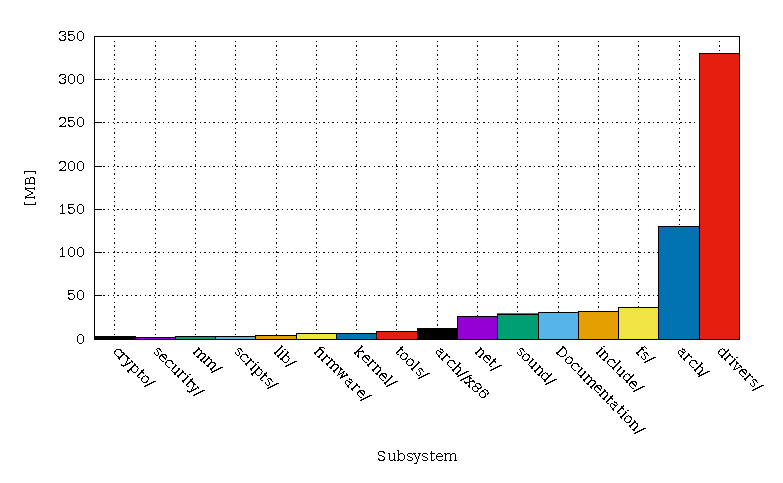
\includegraphics{plots/subsystemsizes.eps}
% \figb{Visualization of the sizes of the subsystems}{fig:subsystems}
% ---

The \texttt{drivers/} subsystem is by far the largest subsystem (with 57\% of 
the total lines of code). It contains all device drivers. It is also mostly 
contributed to by hardware vendors, who want their hardware to be able to run 
on Linux.
\\

The \texttt{arch/} subsystem (18\%) contains architecture specific source code. 
There are 29 folders in the \texttt{arch/} subsystem. One for each major 
architecture that is supported. To highlight a few, the \texttt{x86} 
architecture is used for most common personal computers, the \texttt{arm} 
architecture is used mostly for mobile devices, and the \texttt{powerpc} 
architecture has been used for video game consoles.

In this project, only the \texttt{x86} architecture will be used.
\\

The \texttt{fs/} subsystem (6\%) is code regarding filesystems, the 
\texttt{net/} subsystem (5\%) is about networking, the \texttt{mm/} 
subsystem (.6\%) is about memory management, the \texttt{block/} subsystem 
(.2\%) is drivers for data storage devices, and \texttt{include/} (4\%) 
contains \emph{header} files, which the kernel needs when 
compiling\cite{linuxorg}.
\\

Then there are \texttt{sound/}(5\%),  \texttt{kernel/} 
(1\%), \texttt{crypto/} (.4\%), \texttt{security/}  (.4\%), \texttt{lib/} 
(.6\%), and \texttt{block/} (.2\%).
\\

Other smaller subsystems are:

\texttt{virt/}, \texttt{ipc/}, \texttt{init/}, \texttt{firmware/}, and \texttt{usr/}.
\\

And infrastructure subsystems are:

\texttt{tools/}, \texttt{scripts/}, and \texttt{samples/}.


% --- Not showing this graph ---
% \figa
%     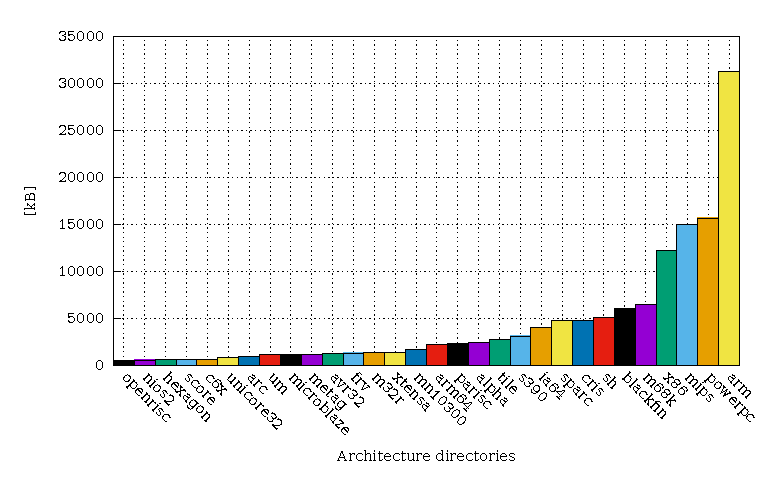
\includegraphics{plots/archsizes.eps}
% \figb{The sizes of the different architecture diretories}{fig:archsizes}
% ---


% TODO
\iffalse
  . talk about allnoconfig alldefconfig in background chapter
  v mention exactly how many configurations there are. (maybe the report 
    from Andrzej). like 2**11,000
  . Find out how to find the exact number of possible configurations. It 
    is in some article, I got by Andrzej. Plus maybe SharpSAT.
  v Write about all the subsystems and what they are for.
  x Explain how to find the number of features by grepping.
  v Maybe talk about the percentage of code in every subsystems. What is 
    Linux kernel made of?
  x talk about who contributes to the kernel. (intel, novell). Both in 
    code and money?
  v mention some more subsystems other than drivers and arch
\fi

            \subsection{The \textsc{Kconfig} language} 
\textsc{Kconfig} is the language of the feature model in Linux (also used for 
other projects like \textsc{BusyBox}, \textsc{BuildRoot}, \textsc{CoreBoot}, 
\textsc{Freetz} and others)\cite[p. 4]{VarModSSD}.

            \def \fn{Found with the command \textcode{find .\ | grep Kconfig | wc}}

The \textsc{Kconfig} files have the prefix \textcode{Kconfig}, and are 
scattered all over the Linux kernel source code tree, where they include each 
other. There are 1195 \textsc{Kconfig} files in total in the stable Linux kernel\f
with 956 of them relevant for the \texttt{x86} architecture.
\\

The corresponding \textsc{Kconfig} code for the phone example in Figure 
\ref{featurediagramphone} can be seen in Figure \ref{kconfigphone}. It 
is a simple example, which lacks some of the possible data types, and other 
syntax available in \textsc{Kconfig}.

For a description of the context free grammar of 
the \textsc{Kconfig} language, see the Appendix \ref{app:kconfig}.
\\

            \def \fn {The percentages are of the 10,335 features available for 
                the \texttt{x86} architecture}

The different data types in the Kconfig language used in Linux are 
\textcode{boolean} (35\%)\f, 
\textcode{tristate} (61\%), \textcode{string} (0.41\%), \textcode{hex} 
(0.32\%), and \textcode{integer} (3.7\%). \texttt{tristate} is a datatype 
with three possible values: \texttt{y},\texttt{n}, and \texttt{m}, where 
\texttt{m} will set the feature as a module instead of building it into the 
kernel. It can then be loaded into the kernel when installing and running the 
kernel.

This does not mean that \texttt{m} and \texttt{n} will be the same in this 
project.




\figa
    \subfigure{
        \lstinputlisting[]{code/kconfigphone}
    }
\figb{\textsc{Kconfig} code for the phone example}{kconfigphone}


%TODO
\iffalse
  v Explain the Kconfig language a bit
  . Reference to Thorsten's projects
  . Refer to the /Documentation/kbuild/kconfig-language.txt
  v Should I have the Backus Naur Form of the Kconfig language here?
\fi


            \subsection{Configuring Linux}
            \label{sec:conf}

The Linux kernel comes with different ways of choosing features - these are 
called \emph{configurators}. 

Some of them lets the user choose the features. There is a question based 
one: \texttt{config}, and some menu based ones: \texttt{menuconfig}, 
\texttt{xconfig}, \texttt{nconfig}, and \texttt{gconfig}.
\\

Figure \ref{fig:lineofconfigs} shows what the graphical 
configurators \texttt{menuconfig} and 
\texttt{xconfig} look like.
\\


\figa
    \includegraphics[scale=0.25]{pngs/2configs.png}
\figb{\texttt{menuconfig} and \texttt{xconfig}}{fig:lineofconfigs}

Other configurators will 
never prompt the user for anything, but create a configuration automatically: 
\begin{itemize}
    \item \texttt{allyesconfig} (enabling as much as possible) 
    \item \texttt{allnoconfig} (disabling as much as possible)
    \item \texttt{tinyconfig} (same as \texttt{allnoconfig} but with higher 
    compression rate, to fit on smaller devices.
    \item \texttt{defconfig} (choosing the default values for everything)
    \item \texttt{randconfig} (choosing random values for everything).
\end{itemize}


When a configuration file is generated, it is saved as \texttt{.config}.
In this file, all features are prefixed with \texttt{CONFIG\_}, and this is
the configuration of the Linux kernel. 

Running the configurator \texttt{allnoconfig} on the \textsc{Kconfig} code for 
the phone example will disable all the features 
in the feature model that can be disabled. Figure \ref{lst:allnoconfig} shows 
the \texttt{.config} file that will be generated when running 
\texttt{allnoconfig}.
\\

The \texttt{CALLS} and \texttt{SCREEN} are mandatory, and will 
therefore be enabled. Out of the three possibilities in the choice clause, the 
\texttt{HD} feature has been enabled, since it is the default choice. Everything
else is disabled.


\figa
    \subfigure[allnoconfig]{
        \label{lst:allnoconfig}
        \lstinputlisting[firstline=5]{code/allnoconfig}
    }
    \qquad %spacing
    \subfigure[allyesconfig]{
        \label{lst:allyesconfig}
        \lstinputlisting[firstline=5]{code/allyesconfig}
    }
\figb{}{}


Figure \ref{lst:allyesconfig} shows the \texttt{.config} file that is generated by 
the configurator \texttt{allyesconfig}.

Every feature has been enabled, except \texttt{COLOR} and \texttt{BW}, which 
must be disabled because only one feature within the choice clause can be enabled.
\\

Running \texttt{allnoconfig} on the Linux kernel, will enable 228 features and 
\texttt{allyesconfig} will enable 6976 features.


            %%% COMPILING AND CATCHING WARNINGS
            \subsection{Compiling and Catching Warnings}

When the Linux kernel has been configured, it is ready to be compiled to create 
the executable kernel. The compiler will then only include the code parts, 
which are indicated by the configuration file. This is written in the source 
code as \textcode{\#ifdef CONFIG\_FOO}.

When writing code for variability software, a programmer has to be aware of the 
\textcode{\#ifdef} clauses, and that different configurations can exist, which 
will only enable some of the code. A programmer can fail to check all possible 
configurations when writing the code, and accidentally make coding mistakes.
\\

When compiling the Linux kernel, the command \textcode{make all} is run, and 
this will start the compilation. If any warnings or errors happen, they will be 
posted in the standard output in the terminal.
\\

In a warning output, there is information about a possible coding mistake that 
might break the code. There are 100s of different warning types, that can be 
enabled. 33 of the these can be enabled by giving the \textcode{-Wall} flag 
to the compiler \textsc{gcc}\cite{gccwarnings}. This will enable warnings 
\emph{"about contructions that some users consider 
questionable"}\cite{gccwarnings}.



            %%% GCC WARNINGS
            \subsection{\textsc{gcc} Warnings}
            \label{sec:gccwarns}
All experiments are run with the \textsc{gcc}-flag \textcode{-Wall}. In many 
cases, though, the Linux kernel enables even more warning flags by itself, and
many of the warnings in the results are not from the \texttt{-Wall} group.
\\

The warnings will be categorized into these types of warnings:

\begin{enumerate}
    \item \textbf{Wrong value warnings}

These warnings will have a chance of breaking the code by returning a wrong
value or doing wrong logic.

    \item \textbf{Code pollution warnings}

These warnings will not break the code, or return wrong data, merely be 
unused code. This plays a role in fitting the Linux kernel on devices with 
space limitations (such as embedded devices).

It can confuse other programmers, who think the code is being used.

    \item \textbf{Bad code practice warnings}

These warnings are deemed unsevere. This does not mean, that they can not be 
severe in other projects, it is usually a heads up to the programmer, that some 
bad practices have been used.

This can also contribute to confusing programmers, who might misunderstand the 
logic.


    \item \textbf{Irrelevant warnings}

These are unsevere warning types.

\end{enumerate}


Here follows a list of the different warning types that was found during the 
experiment.  They are ordered alphabetically, and when code snippets from the 
Linux kernel are present, they are simpilified.


            \subsection*{array-bounds}
This warning is given, when \textsc{gcc} is certain that a subscript to an array is always 
out of bounds.

This will be categorized as a \emph{wrong data} warning.

% See example in figure \ref{lst:arraybounds}.

% \figa
    % \lstinputlisting[language=C]{code/arraybounds}
% \figb{}{lst:arraybounds}


            \subsection*{cpp}
This shows \textcode{\#warning} directives written in the code. This is a warning
message that the coder can pass to the compilee. Often they will not result in 
an error, but inform about specifics.

This is categorized as \emph{irrelevant}.


            \subsection*{deprecated-declarations}
This will show a warning when a function is used, which a programmer has 
declared deprecated. This typically means that a function is run, which is old
and has been replaced - or has not yet been replaced - by another function.

This is categorized as a \emph{wrong data} warning.


            \subsection*{frame-larger-than=NUMBER}
This is a warning that the stack frame is larger than NUMBER.

This is categorized as \emph{irrelevant}.


            \subsection*{implicit-function-declaration}
This is given, when a a function has not been declared, but is being used.

This is categorized as \emph{bad code practice}.


            \iffalse % --- only in gcc 5.9

            \subsection*{incompatible-pointer-types}
This shows when there is converted between pointers, which have incompatible 
types.

This is categorized as a \emph{wrong data} warning.

            \fi % ---


            \iffalse % --- only in gcc 5.2

            \subsection*{int-conversion}
This warns about incompatible conversions between integers and pointers.

This is categorized as \emph{wrong data}.

            \fi % ---

            \subsection*{int-to-pointer-cast}
This warns about an integer being cast to a pointer with a different size.

This will be categorized as \emph{wrong data}.


            \iffalse % --- This was only in gcc 5.2

            \subsection*{logical-not-parentheses}
This warning occurs when the left hand side of an expression contains a 
\emph{logical not} (a \texttt{!} in C). An example is 
    \textcode{if (!ret == template[i].fail)} 
from the file \texttt{crypto/testmgr.c}.

The statement can be interpreted in these 2 ways, which do not necessarily mean 
the same in all cases:

\begin{itemize}
    \item \textcode{!\ (ret == template[i].fail)} 
    \item \textcode{(!ret) == template[i].fail}
\end{itemize}

This is categorized as \emph{wrong data}.

            \fi % --- 17 lines up


            \subsection*{maybe-uninitialized}
This warning is related to the \emph{uninitialized} warning. This shows when 
there is an uncertainty about a variable being uninitialized. In the 
case in Figure \ref{lst:maybeuninitializedreal} there is a \texttt{switch-case} 
where the variable \textcode{sgn} is not initialized in all of the cases.

If \textsc{gcc} cannot see for sure that the variable is initialized, it will 
return this warning.

\figa
    \subfigure{
        \lstinputlisting[language=C]{code/maybeuninitializedreal}
    }
\figb{A real example of maybe-uninitialized function}{lst:maybeuninitializedreal}

This is categorized as \emph{wrong data}.


            \subsection*{overflow}
This is when an integer is truncated into an unsigned type. This can lead to 
wrong data, and is categorized as a \emph{wrong data} warning.


            \subsection*{pointer-to-int-cast}
This warns about a pointer being cast to an integer with a different size.

This will be categorized as \emph{wrong data}.


            \subsection*{return-type}
This will be shown when there is a non-void function, which has no return 
statement.

This is categorized as a \emph{bad code practice} warning.
% TODO: is it really?


            \iffalse % --- Was only in gcc 5.2

            \subsection*{switch-bool}
This warning is shown when a \texttt{boolean} is used in a \texttt{switch} 
statement. When dealing with a \texttt{boolean}, an \texttt{if} statement 
should suffice, and this warning might indicate that the wrong variable is used.

This is categorized as \emph{wrong data}.

            \fi % ---

            \subsection*{uninitialized}
This warns about uninitialized variables. The variable has been declared, but 
has not yet been given a value.

This is categorized as a \emph{wrong data} warning.


            \subsection*{unused-function}
This is a warning about a function, which has been declared and initialized, 
but has never been called. 

This is categorized as \emph{code pollution}.
\\

In the example in Figure \ref{lst:unusedfuncreal}, the function 
\texttt{bq27x00\_powersupply\_unregister} will only be called if the feature 
\texttt{CONFIG\_BATTERY\_BQ27X00\_I2C} is enabled, and is therefore an 
unused function.

\figa
    \lstinputlisting[language=C]{code/unusedfuncreal}
\figb{A real example of an unused function - from the file 
    \texttt{drivers/power/bq27x00\_battery.c}}{lst:unusedfuncreal}


            \subsection*{unused-variable}
This is the same as \texttt{unused-function}, but only with a variable instead 
of a function. There will be no example of this.

It is also categorized as \emph{code pollution}.


            \subsection*{unused-label}
This is the same as the \texttt{unused-function} and \texttt{unused-variable} 
warnings with a label instead.

This is categorized as \emph{code pollution}.




%%%%%%%%%%%%%%%%%%%%%%%%%%%%%%%%%%%%%%%%%%%%%%%%%%%%%%%%%%%%%%%%%%%%%%%%%%%%%%%%
%                           METHODOLOGY
%%%%%%%%%%%%%%%%%%%%%%%%%%%%%%%%%%%%%%%%%%%%%%%%%%%%%%%%%%%%%%%%%%%%%%%%%%%%%%%%
\newpage
\chapter{Methodology}

\emph{Objective:}
This report aims to make a quantitative analysis of warnings in all of the
Linux kernel by checking randomly generated Linux kernels for warnings and 
then generalize.
%The warnings functions as a proxy for errors.

This includes addressing the following research questions:
\\

\textbf{RQ1:} What warnings are the most common in the stable Linux kernel?
\\

\textbf{RQ2:} Where do most warnings occur?
\\

\textbf{RQ3:} Are there any significant differences between an in-development 
version of Linux and a stable version?
\\

\emph{Subject:}
To respond to these questions there will be generated random configurations, 
and these will be used to compile two different versions of the Linux kernel, 
the latest stable Linux kernel version, and some two months old in-development 
versions of the Linux kernel.

The warning messages will be categorized and collected, and be subject for 
analysis.
\\

\emph{Methodology:}
The methodology will be in three parts. First part is finding a way of
generating random configurations in a representative way. Second part is 
collecting any warnings that a compilation might return. Third part is 
analyzing the data and answering the research questions.
\\

        \def \fn{Not counting cross-tree contraints, but also saying 
        everything is a \texttt{boolean} and not \texttt{tristate}, or 
        \texttt{string}.}

For the configurations to be representative every configuration must be equally 
likely to get generated as others in the configuration space. But since there are more than 
10,000 different features in the feature model of the Linux kernel, there will 
be approximately $2^{10,000}$ ($=10^{3080}$) possible configurations in the 
configuration space, assuming the feature model is 100\% \texttt{boolean}s and 
there are no cross-constraints.  This is more than the estimated number of 
atoms in the universe, so getting a list of all the possible configurations is 
not possible (at least not with today's computers).
\\

This means that there might be a generalization problem, and a clever way of 
generating configurations will have to be found. See Section \ref{rephunt}.



            %% EXPERIMENTAL SETUP
            \section{Experimental Setup}
The experimental setup consists of a loop, which does three things. \emph{1:} a 
configuration is generated, \emph{2:} the Linux kernel is then compiled with 
this configuration, and \emph{3:} the output warnings are categorized and 
collected.

Notice that the Linux kernels are not installed and executed in the experiment.
\\

The experiment is mainly carried out on a computer at the IT University of 
Copenhagen. The computer has a $32\times2.8 MHz$ cpu and $128 GB$ of RAM, and 
the average time to run an experiment loop is around 1 minute and 35 seconds. 
Also a conventional laptop with a $4\times2.5 MHz$  cpu and 4 GB of RAM has 
been used. The experiment runs for little over a month.
\\


To say something about all of the Linux kernel, the generated configurations 
in part one of the experiment  should be a representative sample of all the 
possible configurations. 
\\


In Figure \ref{fig:reprrand} a blue area represents the whole configuration 
space, and red dots inside a blue area represent a subset of all the 
configurations, which is in a given sample.
\\

Figure \ref{fig:repr} shows a sample, which is represesentatively distributed 
over the configuration space. 
\\

Figure \ref{fig:rand} shows a sample, which is not representatively 
distributed. All the dots tend to cluster together around certain areas of the 
configuration space, and if one was to tell what the configuration space looked 
like by only looking at the sample, it would look like the yellow area.

\figa
    \subfigure[A representative sample]{
        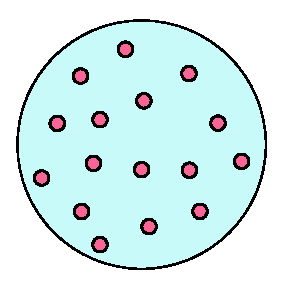
\includegraphics{svg/repr.eps}
        \label{fig:repr}
    }
    \subfigure[An unrepresentative sample]{
        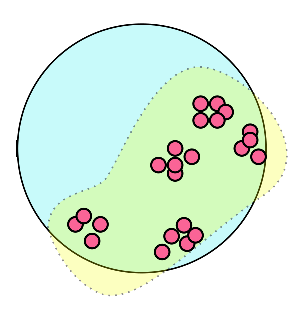
\includegraphics{svg/rand.eps}
        \label{fig:rand}
    }
\figb{Showing both representative (a) and unrepresentative (b) samples}{fig:reprrand}



        %% PART 1: CHOOSING THE CONFIGURATOR
        \section{Part 1: The Hunt For Representativeness}
        \label{rephunt}


Five different methods are proposed and discussed to generate random 
configurations.

\begin{enumerate}

    \item \textbf{Using randconfig}

Using the built-in \texttt{randconfig} configurator.

This comes out of the box with Linux, and always generates valid configurations,
and does so in a few seconds. A caveat is that it does not generate the 
configurations representatively. Read section \ref{sec:randconfbias} about how 
\texttt{randconfig} is not representative.


    \item \textbf{Changing randconfig}

This method will rewrite the code for \texttt{randconfig} or create a new 
configurator (eg. \texttt{reprandconfig}).  This configurator must not have the 
bias for features in the upper levels of the dependency tree, as 
\texttt{randconfig} has.

This would require good knowledge of programming in the \textsc{C} language
and also an algorithmic way of estimating the number of features in all the 
subtrees.


    \item \textbf{Permuting \textsc{Kconfig}}


This proposal will desugarize the \textsc{Kconfig} files to be in one level 
only, by replacing \textcode{if FOO ... endif} clauses by \textcode{depends on} 
options in the features clauses, and then randomly scramble the position of 
the feature clauses in the files. After this, \texttt{randconfig} is run.

The hope is that the \texttt{randconfig} script loads the \textsc{Kconfig} 
files from top to bottom, and will then load in the features at random each 
time.


    \item \textbf{Generate and filter}

            \def \fn {It also is aware about \texttt{choice} clauses}

In this method, a configuration file is generated with a script, which 
does not know the relation betweeen all the features. It knows all the feature
names, and the possible values for the features, and is aware of the choice 
clauses.

It goes through the list and randomly selects values for all the features. Then 
all invalid configurations are filtered away.


    \item \textbf{RandomSAT}

The Linux kernel feature model can be extracted from the \textsc{Kconfig} 
files, to get a propositional formula\cite{lvat}. 

This formula can be used with a SAT solver, which uniformly selects a random
value for all features, which also satisfies the propositional formula, and
thereby always returns a valid random configuration.


    
\end{enumerate}


Out of these five methods, \texttt{randconfig} is selected as a proxy for 
getting a representative sample, on the grounds that the other methods either
do not work as intended, or depends on too much time or expertise to be realistic 
in this project.

\iffalse
  v 4 different ways
  v randconfig
  x fig (a) and (b) showing randconfig
  v Showing the sample figure with dots and stuff.
\fi





            %%% COMPILING AND COLLECTING DATA
            \section{Part 2: Compiling and Collecting Data}

When a configuration file has been generated, two different Linux kernel 
versions are compiled using that configuration file, a stable Linux kernel, and 
an in-development version. The in-development versions are suspected to be more 
prone to contain warnings, but the warnings are also suspected to be fixed 
quicker than the bugs in the stable version. To even out any short-lifed 
warnings, multiple in-development versions are used; nine different versions 
from nine following days.
\\

The kernel is compiled by running the command \textcode{make all}. This command 
runs \textsc{GNU Make}, which is instructed how to compile the kernel with 
\textsc{gcc}. The warning and error outputs from \textsc{gcc} will be saved for analysis.
\\

A warning output will contain a \emph{bug type}, a \emph{filename}, \emph{line 
number}, and a \emph{message} describing the warning in english. This data about the
experiment run is saved: The original error messages, the \texttt{.config} file, 
the Linux version, the \textsc{gcc} version.

This way the experiment will be reproducible.






            %% ANALYZING DATA
            \section{Part 3: Analyzing Data}
The warnings will be quantitatively analyzed.  The analysis of the warnings is 
 quantitative, and this project will not contain in-depth analysis of 
any of the warnings in comparison to\cite{42bugs}, which is a qualitative 
analysis of bugs in Linux.

The analysis is in the next chapter.


%%%%%%%%%%%%%%%%%%%%%%%%%%%%%%%%%%%%%%%%%%%%%%%%%%%%%%%%%%%%%%%%%%%%%%%%%%%%%%%%
%                               RESULTS
%%%%%%%%%%%%%%%%%%%%%%%%%%%%%%%%%%%%%%%%%%%%%%%%%%%%%%%%%%%%%%%%%%%%%%%%%%%%%%%%
\newpage
\chapter{Results}

A total of 42,060 experiments were run. Half of them from the in-development 
Linux version, and the other half of the latest stable version of Linux.

A total of 400,000 warnings were returned with 3,800,000 filenames.
\\

The stable Linux version is analyzed at first, to answer the first two research 
questions. At last, these results are hold against the results from the 
in-development version.


            %% STABLE LINUX WARNINGS
            \section{Stable Linux Warnings}
In Figure \ref{stablewarndis} is shown the distribution of warnings in the 
experiments run with the stable Linux kernel. The distinct warning types are 
only counted once per experiment run.

The warning categories are colored like this: \textred{Wrong data}, 
\textblue{Code pollution}, \textgreen{Bad code practice}, and 
\textgray{irrelevant}.
\\

A total of 245,000 warnings were collected from these experiments, with the 
highest amount of warnings for a single experiment being 111.  Many of the 
warnings found, are the same exact warnings, happening in the same files over 
and over. This is natural, since many different experiments are bound to create 
some of the same warnings, as it all comes from the same code base.
\\

17\% of the compilations stopped with an error. These errors were mostly 
errors, which were specific for the build machine because of missing libraries 
or programs, and will not be looked into.  The compilations that had errors 
were made to stop after the first error was found to not have data pollution 
caused by an avalanche effect.
\\


% TODO
% . Actual number of files, bugs, configs

\figa
    \begin{tabular}{r|d|c}
        \hline
        \hline
        \textbf{Warning} & \multicolumn{1}{|c|}{\textbf{Percentage}} & 
        \textbf{Category}\\
        \hline

            \rowcolor{blue!20}
        {unused-function} & 59. \% & Code pollution \\
            \rowcolor{red!20}
        maybe-uninitialized & 45. \% & Wrong data \\
            \rowcolor{blue!20}
        unused-variable & 29. \% & Code pollution \\
            \rowcolor{gray!30}
        cpp & 24. \% & Irrelevant \\
            \rowcolor{red!20}
        uninitialized & 19. \% & Wrong data \\
            \rowcolor{gray!30}
        ERROR & 17. \%  & Irrelevant \\
            \rowcolor{red!20}
        pointer-to-int-cast & 17.\% & Wrong data \\
            \rowcolor{gray!30}
        frame-larger-than= & 14.\% & Irrelevant \\
            \rowcolor{red!20}
        array-bounds & 11.  \% & Wrong data \\
            \rowcolor{green!20}
        return-type & 7.7 \% & Bad Code Practice \\
            \rowcolor{red!20}
        int-to-pointer-cast & 7.6 \% & Wrong data \\
            \rowcolor{red!20}
        overflow & 6.5 \% & Wrong data \\
            \rowcolor{blue!20}
        unused-label & 5.4 \% & Code Pollution \\
            \rowcolor{red!20}
        deprecated-declarations & 5.4 \% & Wrong data \\
        %error=implicit-function-declaration & 4.6 \% & Irrelevant \\
            \rowcolor{green!20}
        implicit-function-declaration & 5.6 \% & Bad code practice \\ % 4.6 added from 2 lines up.
        %error=implicit-int & 0.029 \% & - \\

        \hline
        \hline
    \end{tabular}
\figb{Distribution of warnings in the stable kernel}{stablewarndis}


The following observations have been made:
\\

\textbf{Observation 1:}
The most common warnings in the \textred{Wrong data} category are: 
\emph{maybe-uninitialized} and \emph{uninitialized}, which are two related 
warnings.
\\

\textbf{Observation 2:}
Two out of three \textblue{code pollution} warnings \emph{unused-function} and 
\emph{unused-variable} are both in the top 3 of most common warnings.
\\

\textbf{Observation 3:}
There are only found 15 different warning types. Only 8 of these are from the 
\texttt{-Wall} group.
\\

With these observations, \textbf{RQ1} can be answered.
\\

\underline{\textbf{Conclusion 1:}}
The warning types that appear the most, are warnings regarding \textblue{code 
pollution}, and next come warning types related to variables being 
uninitialized.


%RQ1: What warnings are the most common in the stable Linux kernel?



            %% STABLE LINUX SUBSYSTEMS
            \section{Stable Linux Subsystems}
Figure \ref{stablessdis} shows the distribution of subsystems with warnings in 
all of the experiment runs on the stable Linux version. In many experiment runs, 
there were multiple warnings in the same subsystems. These are only counted 
once.

The gray rows are subsystems that are not a major part of the kernel 
functionality, as mentioned in  Section \ref{sec:linuxss}. These are the 
\textredmid{smaller} subsystems, and the \textreddark{infrastructure} 
subsystems.
\\


% SQL:
%   set @ss = 'scripts/';
%   select count(distinct config) from bugs
%       where linux_version rlike '4.1.1' and (
%           original rlike concat(' ', @ss) or
%           original rlike concat('^', @ss) or
%           original rlike concat('\\n', @ss) or
%           original rlike concat('\\[', @ss) );


\figa
\subfigure[Percentage of experiment runs]{
    \begin{tabular}{r|d}
        \hline
        \hline
        \textbf{Subsystem} & \multicolumn{1}{c}{\textbf{Percentage}} \\
        \hline
        
        drivers/ &  64. \%  \\
        include/ &  40. \%  \\
        crypto/ &  17. \%  \\
        fs/ &  14. \%  \\ % Same exact number as arch/
            \rowcolor{\reddark}
        {samples/} &  12. \%  \\ % Same exact number as usr/
        net/ &  10. \%  \\
        arch/ &  9.2 \%  \\ % Same exact number as fs/
        arch/x86/ &  9.2 \%  \\ % Same exact number as fs/ and arch/
        lib/ &  9.1 \%  \\
        mm/ &  7.9 \%  \\
        kernel/ &  5.9 \%  \\
        sound/ &  3.8 \%  \\
            \rowcolor{\reddark}
        {scripts/} & 1.6  \% \\
            \rowcolor{\redmid}
        {usr/} &  .076 \%  \\ % Same exact number as samples/
        block/ &  .75  \% \\
        security/ &  .0 \% \\

        \hline
        \hline
    \end{tabular}
} \qquad
\subfigure[Warnings per 1000 lines of code in the subsystem]{
    \begin{tabular}{r|c}
        \hline
        \hline
        \textbf{Subsystem} & \textbf{Warn/kLOC} \\
        \hline

            \rowcolor{\reddark}
        samples/ & 270. \\
            \rowcolor{\reddark}
        scripts/ & 58. \\
        crypto/ & 42. \\
            \rowcolor{\redmid}
        usr/  & 30. \\
        mm/  & 25. \\
        lib/ & 18. \\
        include/ & 13. \\
        arch/x86/ & 8.8 \\
        kernel/ & 2.5 \\
        net/ & 2.4 \\
        fs/ & 2.3 \\
        block/ & 1.5 \\
        drivers/ & 1.2 \\
        arch/ & 0.90 \\
        sound/ & 0.36  \\
        security/ & 0.0 \\

        \hline
        \hline
    \end{tabular}
}
\figb{Distribution of all subsystems within the warnings from the stable Linux}{stablessdis}



With these results,  the following observations can be made:
\\

\textbf{Observation 3:}
The subsystem, which appear the most in the warnings, is the 
\texttt{drivers/} subsystem, followed by the \texttt{include/} subsystem.
\\

\textbf{Observation 4:}
There are zero warnings in the \texttt{security/} subsystem. 
\\

With these observations \textbf{RQ2} can be answered.
\\

\underline{\textbf{Conclusion 2:}}
The subsystems with drivers, and header files have the most warnings, and the 
security subsystem together with the most smaller, and infrastructure subsystems
had zero or near zero warnings.




            %% IN-DEVELOPMENT VERSION VS. STABLE VERSION
            \section{In-Development Version vs.\ Stable Version}


In Figure \ref{comparewarn} is a comparison of the warnings between the stable
version, and the in-development version. Only the 6 warnings out of 15 that 
actually change percentage are shown. All non-shown warnings had less than one 
percent difference between the two versions.


\textbf{Observation 5:}
There are more warnings in the in-development version of Linux, than the stable
version.
\\

\textbf{Observation 6:}
There is only one type of warning that occur more in the stable version, that is
the \texttt{frame-larger-than=} warning.
\\

With these observations \textbf{RQ3} can be answered.
\\

\underline{\textbf{Conclusion 3:}}
There are more warnings and errors in the in-development version.


% TODO 
% Some text in this chapter...

\figa
    \subfigure[Stable version]{
    \begin{tabular}{r|d}
        \hline
        \hline
        \textbf{Warning} & \multicolumn{1}{c}{\textbf{\%}} \\
        \hline

            \rowcolor{blue!20}
        {unused-function} & 59. \% \\
            \rowcolor{blue!20}
        unused-variable & 29. \% \\
            \rowcolor{gray!30}
        ERROR & 17. \%  \\
            \rowcolor{gray!30}
        frame-larger-than= & 14.\% \\
            \rowcolor{red!20}
        int-to-pointer-cast & 7.6 \% \\
            \rowcolor{green!20}
        implicit-function-declaration & 5.6 \% \\

        \hline
        \hline
    \end{tabular}
    }
    \subfigure[In-development version]{
    \begin{tabular}{r|d}
        \hline
        \hline
        \textbf{Warning} & \multicolumn{1}{c}{\textbf{\%}} \\
        \hline

            \rowcolor{blue!20}
        {unused-function} & 62. \% \\
            \rowcolor{blue!20}
        unused-variable & 51. \% \\
            \rowcolor{gray!30}
        ERROR & 38. \%  \\
            \rowcolor{red!20}
        int-to-pointer-cast & 25. \% \\
            \rowcolor{green!20}
        implicit-function-declaration & 23. \% \\
            \rowcolor{gray!30}
        frame-larger-than= & 7.8  \% \\

        \hline
        \hline
    \end{tabular}
    }
\figb{Showing the warning types that has changed more than 1\%}{comparewarn}






\figa
    \subfigure[Stable version]{
    \begin{tabular}{r|d}
        \hline
        \hline
        \textbf{Subsystem} & \multicolumn{1}{c}{\textbf{Percentage}} \\
        \hline
        
        drivers/ &  64. \%  \\
        include/ &  40. \%  \\
        crypto/ &  17. \%  \\
        fs/ &  14. \%  \\ % Same exact number as arch/
            \rowcolor{\reddark}
        {samples/} &  12. \%  \\ % Same exact number as usr/
        net/ &  10. \%  \\
        arch/ &  9.2 \%  \\ % Same exact number as fs/
        arch/x86/ &  9.2 \%  \\ % Same exact number as fs/ and arch/
        lib/ &  9.1 \%  \\
        mm/ &  7.9 \%  \\
        kernel/ &  5.9 \%  \\
        sound/ &  3.8 \%  \\
            \rowcolor{\reddark}
        {scripts/} & 1.6  \% \\
        block/ &  .75  \% \\
            \rowcolor{\redmid}
        {usr/} &  .076 \%  \\ % Same exact number as samples/
        security/ &  .0 \% \\

        \hline
        \hline
    \end{tabular}
    }
    \subfigure[In-development version]{
    \begin{tabular}{r|d}
        \hline
        \hline
        \textbf{Subsystem} & \multicolumn{1}{c}{\textbf{Percentage}} \\
        \hline
        
        drivers/ &  62. \%  \\
        include/ &  42. \%  \\
            \rowcolor{\reddark}
        {scripts/} &  25. \% \\
        crypto/ &  16. \%  \\
        arch/ &  14. \%  \\ % Same exact number as fs/
        arch/x86/ &  14. \%  \\ % Same exact number as fs/ and arch/
        fs/ &  13. \%  \\ % Same exact number as arch/
        mm/ &  13. \%  \\
        net/ &  10. \%  \\
            \rowcolor{\reddark}
        {samples/} & 9.7  \%  \\ % Same exact number as usr/
        lib/ &  9.0 \%  \\
        kernel/ & 3.0  \%  \\
        sound/ &  1.5 \%  \\
        block/ &  .27  \% \\
            \rowcolor{\redmid}
        {usr/} & .12  \%  \\ % Same exact number as samples/
        security/ &  .0 \% \\

        \hline
        \hline
    \end{tabular}
    }
\figb{Comparison of the subsystems}{comparess}






%%%%%%%%%%%%%%%%%%%%%%%%%%%%%%%%%%%%%%%%%%%%%%%%%%%%%%%%%%%%%%%%%%%%%%%%%%%%%%%%
%                           THREATS TO VALIDITY
%%%%%%%%%%%%%%%%%%%%%%%%%%%%%%%%%%%%%%%%%%%%%%%%%%%%%%%%%%%%%%%%%%%%%%%%%%%%%%%%
            \newpage
            \chapter{Threats to Validity}
            \label{ch:ttv}


            %% EXTERNAL VALIDITY
            \section{External Validity}
            \label{sec:extval}


            %%% ONLY ONE ARCHITECTURE
            \subsection{Only One Architecture}

The experiment is only run on the \texttt{x86} architecture. There are more than
20 different architectures supported. For the results to say anything about all 
of the other architectures, a cross-compiler for each architecture will have to
be installed on the building system.

            \def \fn {Can be found here: 
            \url{https://www.kernel.org/pub/tools/crosstool/files/bin/x86_64/4.9.0/}}

This is possible through various scripts, and by installing a new version of
\textsc{gcc} per new architecture\f.



            %% INTERNAL VALIDITY
            \section{Internal Validity}
            \label{sec:intval}

            %% THE BUILT-IN RANDCONFIG
            \subsection{The Built-In \texttt{randconfig} Configurator}
            \label{sec:randconfbias}

The built-in configurator \texttt{randconfig} is not representative, but is 
biased towards features higher up in the feature model tree. 

Figure ~\ref{randconfigtoy} shows a toy example of a \textsc{Kconfig} feature 
model written in the \textsc{Kconfig} language.  It is a very small example 
with only two features, but it will easily explain some limitations of using 
\texttt{randconfig}.
\\

There are two features (\texttt{A} and \texttt{B}) in the example, which can be 
enabled or disabled, and feature \texttt{B} depends on \texttt{A} being enabled.
This leaves three possible outcomes. 

One where both is enabled, one where only \texttt{A} is enabled, and one where 
none of them are enabled. The outcome where only \texttt{B} is enabled is an 
invalid configuration since \texttt{B} depends on \texttt{A}.

\figa
    \subfigure{
        \lstinputlisting[language=C, firstline=1, morekeywords={prompt, config, 
        depends, on, bool, endchoice, choice,{||}}]{code/kconfigrandconfigtoy}
    }
\figb{A toy \textsc{Kconfig} feature model}{randconfigtoy}

Figure \ref{fig:randtoy50} shows how \texttt{randconfig} will decide whether 
the features are enabled or disabled. It always goes from the top of the tree 
and down. So feature \texttt{A} will always be decided for at first. And since 
it is a \texttt{boolean} there will be a fifty fifty chance.
\\

Then it proceeds further down in the dependency tree, and decides for feature
\texttt{B}, which also has a fifty fifty chance.

For the creation to be representative, all the three possible configurations 
should have equal chance of being created (33\%). See Figure 
\ref{fig:randtoy33} for a visualization of how the selection should 
be to be representative.

% --- 68 lines down ---
\figa
    \subfigure[How \texttt{randconfig} will select]{
    \label{fig:randtoy50}
    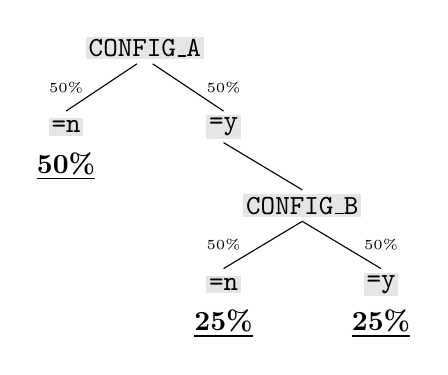
\begin{tikzpicture}
        % Names of configs
        \draw (2,4) node {\textcode{CONFIG\_A}};
        \draw (4,2) node {\textcode{CONFIG\_B}};

        % yeses and nos
        \draw (1,3) node {\textcode{=n}};
        \draw (3,3) node {\textcode{=y}};
        \draw (3,1) node {\textcode{=n}};
        \draw (5,1) node {\textcode{=y}};

        % lines not necessarily from above and down
        \draw[-] (1.9,3.8) edge (1,3.2);
        \draw[-] (2.1,3.8) edge (3,3.2);
        \draw[-] (3,2.8) edge (4,2.2);
        \draw[-] (3,1.2) edge (4,1.8);
        \draw[-] (5,1.2) edge (4,1.8);

        % Draw percentages
        \draw (1,3.5) node {\tiny{50\%}};
        \draw (3,3.5) node {\tiny{50\%}};
        \draw (3,1.5) node {\tiny{50\%}};
        \draw (5,1.5) node {\tiny{50\%}};

        \draw (1,2.5) node {\textbf{\underline{50\%}}};
        \draw (3,0.5) node {\textbf{\underline{25\%}}};
        \draw (5,0.5) node {\textbf{\underline{25\%}}};

    \end{tikzpicture}
    }
% ==== The next graph ====
    \subfigure[Representative selection]{
    \label{fig:randtoy33}
    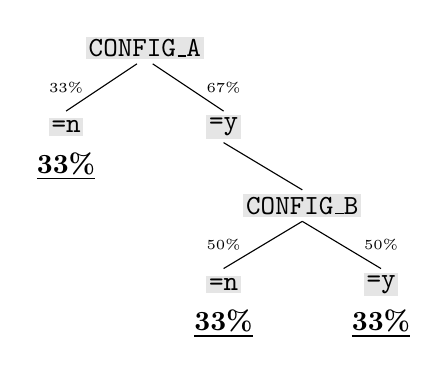
\begin{tikzpicture}

        % Names of configs
        \draw (9,4) node {\textcode{CONFIG\_A}};
        \draw (11,2) node {\textcode{CONFIG\_B}};

        % yeses and nos
        \draw (8,3) node {\textcode{=n}};
        \draw (10,3) node {\textcode{=y}};
        \draw (10,1) node {\textcode{=n}};
        \draw (12,1) node {\textcode{=y}};

        % lines not necessarily from above and down
        \draw[-] (8.9,3.8) edge (8,3.2);
        \draw[-] (9.1,3.8) edge (10,3.2);
        \draw[-] (10,2.8) edge (11,2.2);
        \draw[-] (10,1.2) edge (11,1.8);
        \draw[-] (12,1.2) edge (11,1.8);

        % Draw percentages
        \draw (8,3.5) node {\tiny{33\%}};
        \draw (10,3.5) node {\tiny{67\%}};
        \draw (10,1.5) node {\tiny{50\%}};
        \draw (12,1.5) node {\tiny{50\%}};

        \draw (8,2.5) node {\textbf{\underline{33\%}}};
        \draw (10,0.5) node {\textbf{\underline{33\%}}};
        \draw (12,0.5) node {\textbf{\underline{33\%}}};
    \end{tikzpicture}
    }
\figb{}{}
% --- 68 lines up ---

Representativeness is not of high prioritization for the Linux kernel 
developers, the \texttt{randconfig} function is merely used as a simple fuzz 
testing tool.

This ultimately means that \texttt{randconfig} is not representative in its 
configuration creation. (See more about representativeness in the section 
\ref{rephunt}.)
\\



            %%% MULTIPLE IN_DEVELOPMENT VERSIONS
            \subsection{Multiple In-Development Versions}

Multiple different in-development versions of the Linux kernel are used to 
minimize the skewing of warnings. If only one version of the in-development 
version is used, it gives a very one-sighted view of the in-development 
versions, where certain bugs may be over-represented. The more different 
versions of the in-development Linux should be used, to get a more uniform 
results.

In this experiment, nine different versions of the in-development version was 
used, which is not a lot. Therefore there may be an overrepresentation of 
some warnings in the in-development version results.


            %%% MORE FEATURES IN THE IN-DEVELOPMENT VERSION
            \subsection{More Features in the In-Development version}
In the in-development Linux version, there are 20 more features than in the 
stable version. The configurations are created in the in-development version, 
and are copied over to the stable version. This will result in some unknown 
features being set on the stable version, but there is no code corresponding to 
the features, so no harm is done.

If they are created in the stable version, instead, they will never be given 
random values, but always default values, which will skew the results.
\\


            %%% GCC VERSIONS
            \subsection{\textsc{gcc} Versions}
Roughly a third of the compilations were done with GCC version 5.1.0 and two 
thirds with GCC version 4.9.2. This should not matter on what warnings are 
returned. There is only one new warning that is enabled by the \texttt{-Wall} 
flag in version 5.1.0 (\texttt{-Wc++14compat}), and none of this type was found.
\\

The warnings \texttt{discarded-array-qualifiers}, 
\texttt{incompatible-pointer-types}, \texttt{int-conversion}, 
\texttt{logical-not-parentheses}, and \texttt{switch-bool} showed only on the 
experiments with the newer version of \textsc{gcc}. These warnings were 
discarded from the results.
\\

There is a possibility though, that the newer version is better at finding 
certain warnings that are in the results. This will not be clear to see in the 
data.



            %%% FIRMWARE
            \subsection{Firmware}
When building certain firmware drivers in Linux, external proprietary drivers 
are needed, before they can be built. This firmware is not in the kernelcode, 
but must be downloaded from the hardware vendors homepages.
\\

There are libraries on the internet which contain these firmware drivers, but 
in this report, they will not be included. These drivers are in a sense not a 
part of the open source Linux kernel, and are out of scope with this report.
\\

To disable configurations, which would require these proprietary firmware 
drivers, the following features were given a fixed value in the configurations:

\begin{itemize}
    \item \textcode{CONFIG\_STANDALONE=y}
    \item \textcode{CONFIG\_FW\_LOADER=n}
    \item \textcode{CONFIG\_PREVENT\_FIRMWARE\_BUILD=y}
\end{itemize}


Also every feature that had some relation to the \textsc{z4c} library has been 
disabled, since it was not installed on the build system.

So all features, which were related to the \textsc{z4c} library were also given 
a fixed value.

\begin{itemize}
    \item \textcode{CONFIG\_*LZ4*=n}
\end{itemize}


Furthermore this feature is fixed, since it is also dependent on a library not 
installed on the build system.

\begin{itemize}
    \item \textcode{CONFIG\_SECCOMP=y}
\end{itemize}



% TODO
% . coccinelle
% . Coverity 


%%%%%%%%%%%%%%%%%%%%%%%%%%%%%%%%%%%%%%%%%%%%%%%%%%%%%%%%%%%%%%%%%%%%%%%%%%%%%%%%
%                       FUTURE WORK
%%%%%%%%%%%%%%%%%%%%%%%%%%%%%%%%%%%%%%%%%%%%%%%%%%%%%%%%%%%%%%%%%%%%%%%%%%%%%%%%
            \newpage
            \chapter{Future Work}

            %% MORE THAN LINUX
            \subsection*{More Than Linux}

            \def \fn {\url{http://vbdb.itu.dk/}}

This experiment only runs on the linux kernel, but there are variability in many
other software products. A similar experiment could be run on other products to 
see it the results correlate. The paper \cite{42bugs} has an attached online 
database of the variability bugs found in the paper. These bugs are from both 
the Linux kernel and also \textsc{BusyBox}\f.

            %% OTHER COMPILERS
            \subsection*{Other Compilers}
            

            \def \fn {\url{http://clang.llvm.org/}}

There has been some disputes between the Linux community and the \textsc{gcc} 
creators\cite{linusgcc}. The Linux is often not too happy with how \textsc{gcc} 
handles warnings, and in the last couple of years, there has been an initiative 
to deprecate \textsc{gcc} as the standard compiler for Linux, and instead use 
\textsc{LLVM Clang}\f, which is faster, and has good static analysis\cite{clang}.


            %%  ANALYZE WARNING PRONE FEATURES
            \subsection*{Analyze Warning-Prone Features}

This experiment can be extended to look at what features, or combination of 
features that result in warnings. When the same warning appears in the same 
file, on different configurations, it must necessarily be the same combination 
of a few features that generated the warning. Finding the features that all these
configurations have in common will give a lead to what feature combination is 
creating the warning.

It will be possible to narrow down which features might be generating the bug.


            %% ANALYZE ERRORS
            \subsection*{Analyze errors}

In this project, only warnings could be automatically quantified, because of the
nature of the errors that occured was due to the build system's missing 
dependencies, and also due to the experiment sample not being large enough to 
find many errors.


%%%%%%%%%%%%%%%%%%%%%%%%%%%%%%%%%%%%%%%%%%%%%%%%%%%%%%%%%%%%%%%%%%%%%%%%%%%%%%%%
%                           RELATED WORK
%%%%%%%%%%%%%%%%%%%%%%%%%%%%%%%%%%%%%%%%%%%%%%%%%%%%%%%%%%%%%%%%%%%%%%%%%%%%%%%%
            \newpage
            \chapter{Related Work}

            \subsection*{Variability bugs}
The paper \emph{42 Variability Bugs in the Linux Kernel...}\cite{42bugs} is 
looking at bugs in the linux kernel from a qualitative angle rather than 
quantitative.  The bugs are manually analysed, and discussed.

This report is somewhat a continuation of the research in that paper, trying to 
quantify the warnings part of the bugs.


            %%%  INTEL AND THE KBUILD_ROBOT
            \subsection*{Intel and the Kbuild-Robot}

\textsc{Intel} is a large hardware vendor, which is one of the top ten 
contributors to the Linux kernel\cite{gkh}. They have started a bugfix 
initiative called \texttt{Kbuild-robot}, which every day runs part 1, and part 
2 of this experiment on the in-development version of Linux. As a part 3 and 4, 
some of the kernels are run, and when an error is found, the author of the change 
is notified with an e-mail.

The mailing lists are publicly available at 
\cite{kbuildrobot,kbuildrobotall,kbuildlkp}.
\\

What is gathered of information about the \texttt{kbuild-robot} project, only 
the mailing lists are publicly available, and the experiment run data is thrown 
away soon after. 

According to \cite{summit2012,summit2013}, 30,000 kernels are compiled and run
each day. That is about the same amount of experiment runs this project does in 
a month.

An effort was made to get their experiment data available for analysis, but no 
luck.  




% TODO
\iffalse
  \ 42 bugs
  . Variability in ...
  . Paper from Iago
  v Fengguang Wu and Intel
  v Jaccard Similarity (?)
  . http://codemonkey.org.uk/tag/coverity/ <- Correlate data with this guys drivers/staging thing.
\fi



%%%%%%%%%%%%%%%%%%%%%%%%%%%%%%%%%%%%%%%%%%%%%%%%%%%%%%%%%%%%%%%%%%%%%%%%%%%%%%%%
%                    CONCLUSION
%%%%%%%%%%%%%%%%%%%%%%%%%%%%%%%%%%%%%%%%%%%%%%%%%%%%%%%%%%%%%%%%%%%%%%%%%%%%%%%%
            \newpage
            \chapter{Conclusion}
The Linux kernel has been analyzed, and there are 14 different 
warnings that appear in the Linux kernel. The majority of these are regarding 
code pollution, and uninitialized variables.
\\

The \texttt{drivers/} subsystem has the most warnings, but there are warnings 
in the most subsystems with exception of some of the smaller subsystems and 
infrastructure subsystems, and also no warnings were found in the 
\texttt{security/} subsystem.
\\

In the in-development version of Linux, there are generally more warnings (and
errors) than in the stable version. Half of the warnings appear about the same
amount of the experiment runs, while the other half appear almost double as 
many times.




\newpage
\bibliographystyle{siam}
\bibliography{bib}


%%%%%%%%%%%%%%%%%%%%%%%%%%%%%%%%%%%%%%%%%%%%%%%%%%%%%%%%%%%%%%%%%%%%%%%%%%%%%%%%
%                           APPENDIX
%%%%%%%%%%%%%%%%%%%%%%%%%%%%%%%%%%%%%%%%%%%%%%%%%%%%%%%%%%%%%%%%%%%%%%%%%%%%%%%%
            \newpage
            \chapter{Appendices}


            %%% KCONFIG LANGUAGE
            \section{\textsc{Kconfig} language}
            \label{app:kconfig}

            \def \fn {\url{http://www.lua.org/manual/5.1/manual.html}}

Following is the \textsc{Kconfig} language context free grammar in the 
\emph{Backus Naur Form} inspired by the \textsc{Lua} documentation\f.

% KCONFIG BACKUS NAUR FORM --- 34 lines down
\begin{verbatim}
stat ::= 'config ' id '\n' options

id ::= characters { characters }

characters ::= [A-Za-z_0-9]\*

options ::= mandatory optional

types ::= 'bool' | 'boolean' | 'tristate' | 'int' | 'string' | 'hex'
deftypes ::= ( 'def_bool' | 'def_tristate' ) expr

mandatory ::= types [ '"' characters '"' ] [ expr ] |

optional ::= 'depends on ' expr
             'select ' expr
             'help\n' characters

expr ::= id [ '=' characters ] 
         expr '&&' expr |
         expr '||' expr |
         '(' expr ')'
         'if ' expr
         'menu' text
         'y'
         'n'

text ::= characters | symbols 
         text text

symbols ::= '/-(),.'

\end{verbatim}
% --- 34 lines up


            %%%%%%%%%%%%%%%%%%%%%%%%%%%
            %%      DATA              %
            %%%%%%%%%%%%%%%%%%%%%%%%%%%
            %\section{Data}






\end{document}



